\section{Inherently Non-resonant Antenna}
In this section the prototype of the Inherently non-resonant antenna will be described.

The prototype and the used tuning circuit is shown in Figure \ref{fig:ant3techschem_proto}. Both antennas are made on a CNC mill in the AAU metal workshop. This was done in order to have perfectly smooth edges and cut the two-feed design accurately.   

\begin{figure}[htbp]
    \begin{subfigure}[b]{0.49\linewidth}
        \centering
        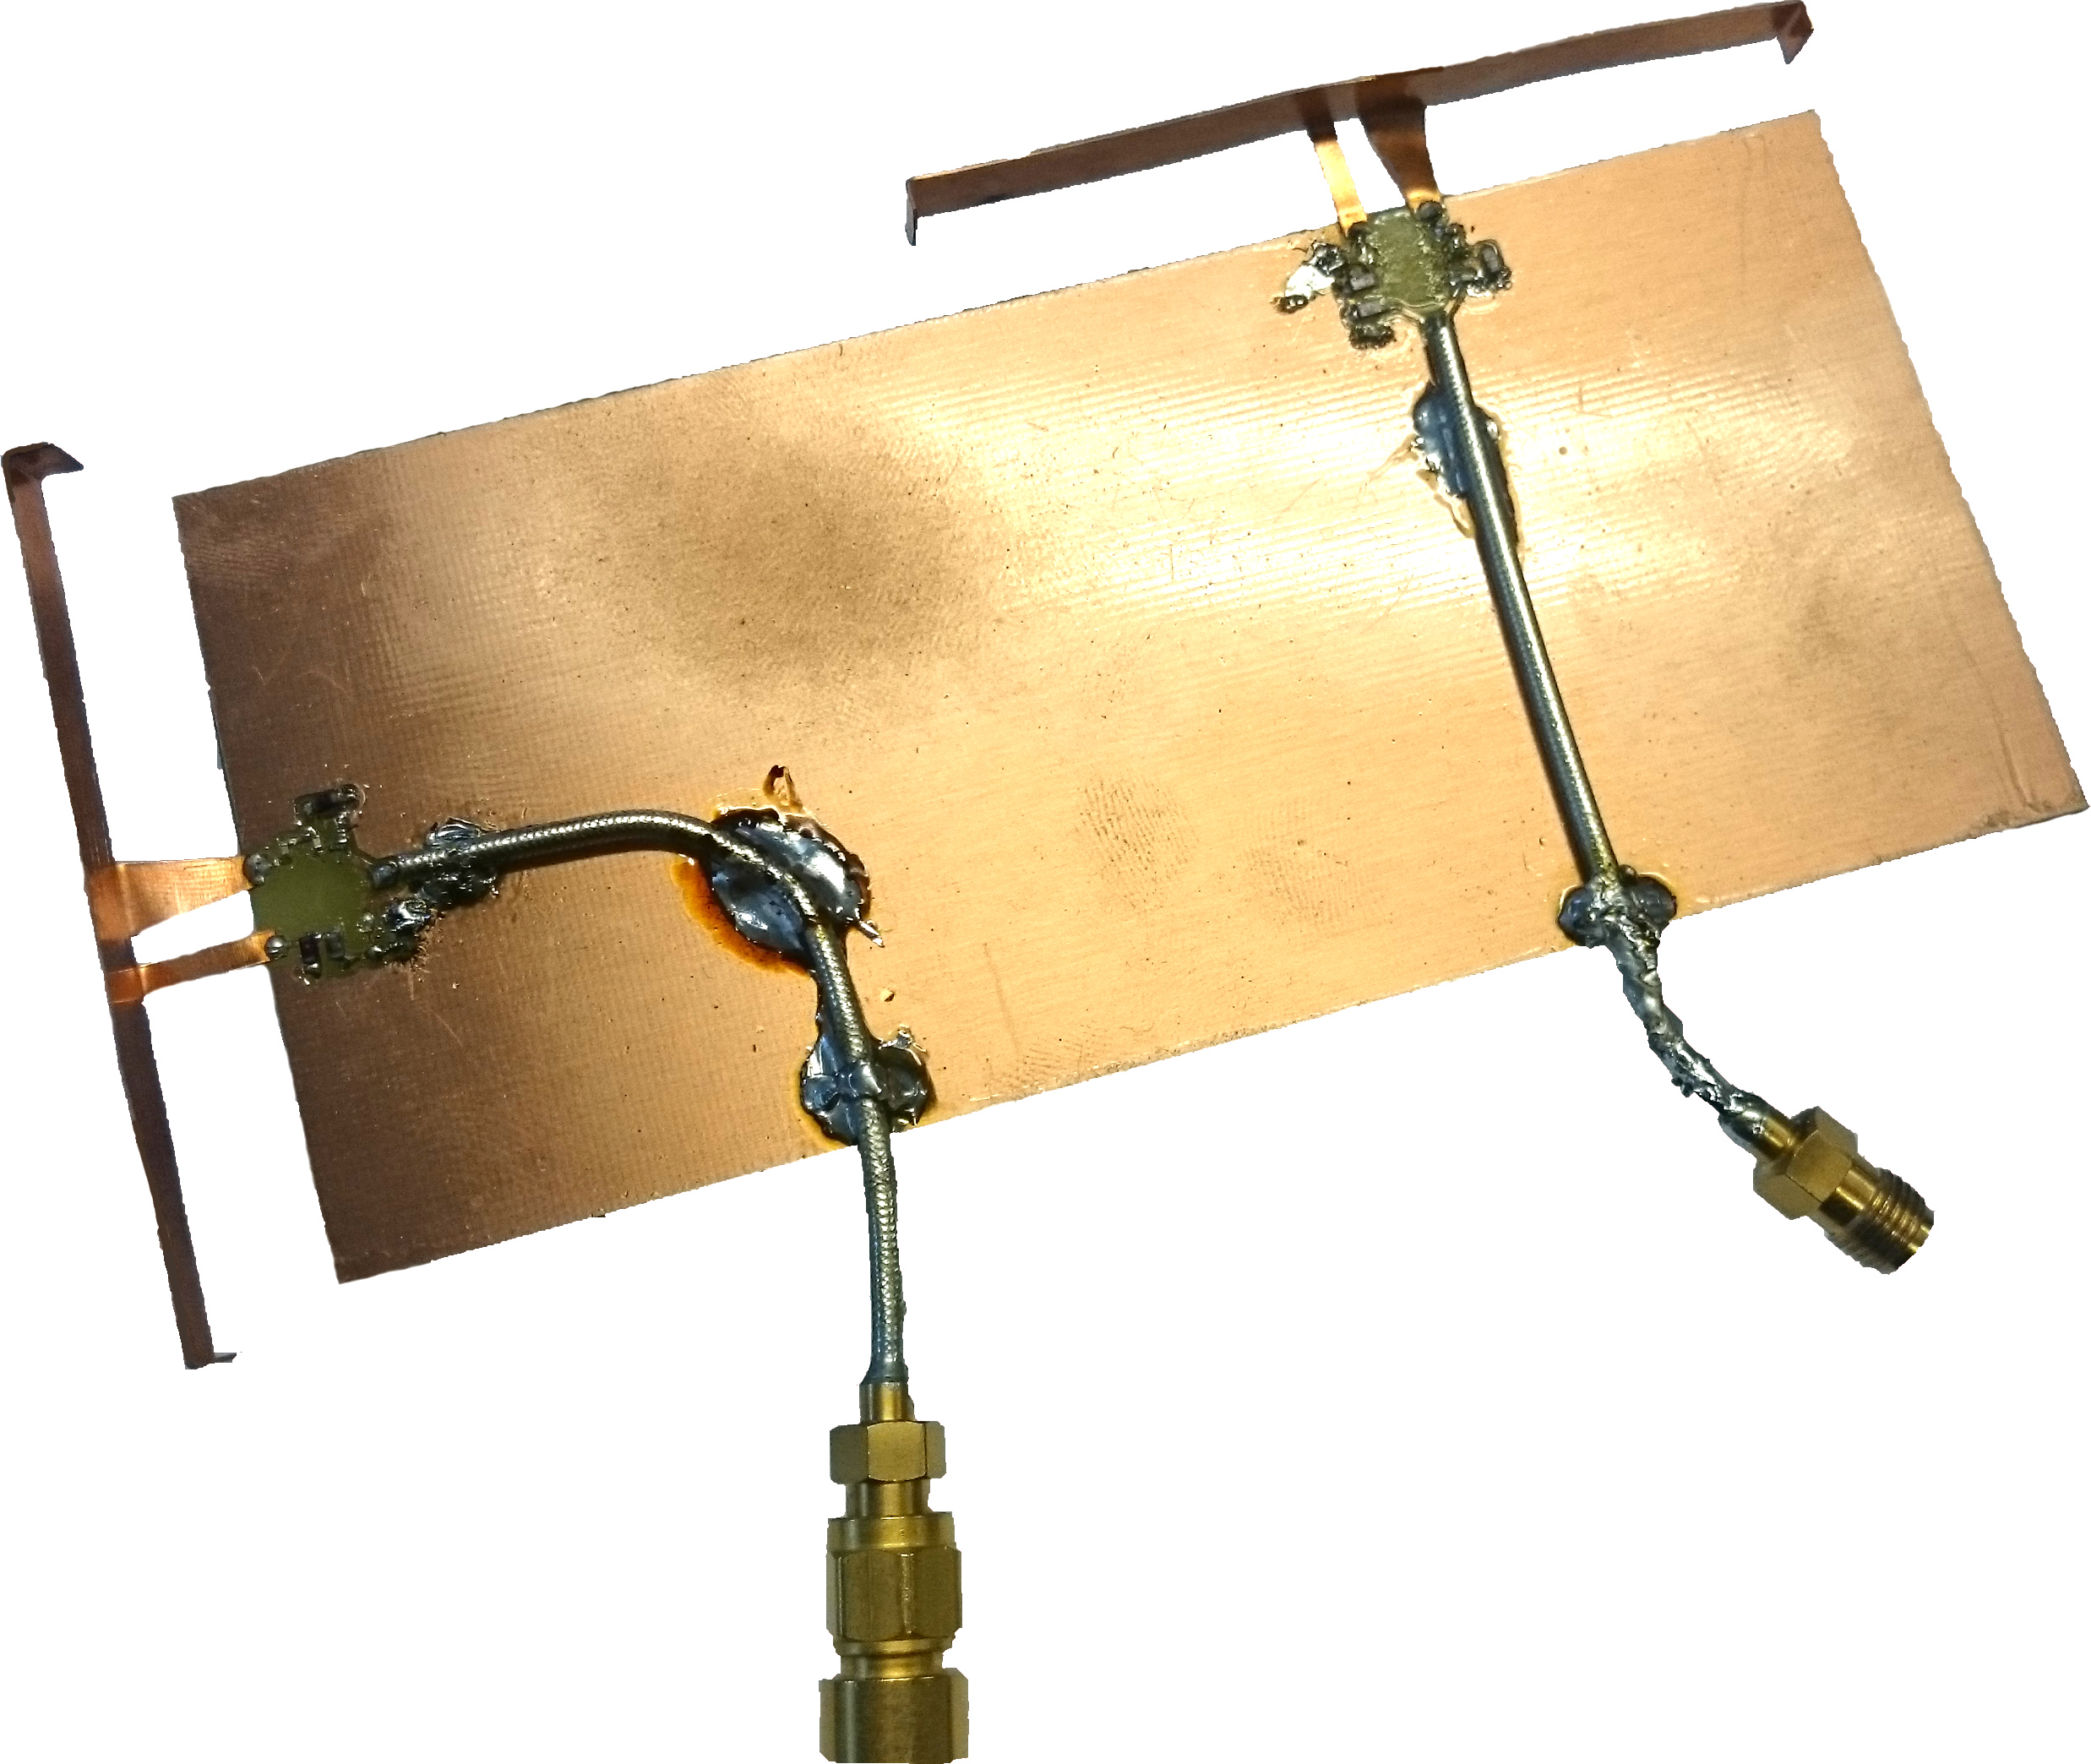
\includegraphics[scale=0.1]{img/tech_sol/nonresonant/prototype/3d_figure.jpg}
        \caption{Non-resonant antenna prototype.}
        \label{fig:nonresonant_proto}
    \end{subfigure}
    \hfill
    \begin{subfigure}[b]{0.49\linewidth}
        \centering
        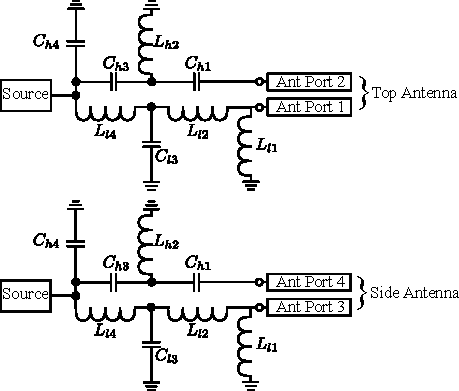
\includegraphics{img/tech_sol/nonresonant/schematic_tuning}\\[0cm]
        \caption{Tuning/matching circuit.}
        \label{fig:ant3schematic}
    \end{subfigure}
    \caption{Picture and tuning circuit for the prototype antenna.  The antennas are built on FR-4 board using \SI{35}{\micro\meter} copper. There is a matching circuit as shown for each of the four feeds.}
    \label{fig:ant3techschem_proto}
\end{figure}


\subsection{Measurement and Simulation Comparison}
The simulated and measured S-parameter and total efficiency is shown in Figure \ref{fig:nonresonant_proto_sparam_eff}. The results are done with the tunable capacitor at \SI{0.3}{pF}. Furthermore some adjustments were done to the component values, the current values can be seen in Table \ref{fig:ant3schematic_proto}. 

From the S-parameter and the bandwidth table it is seen that both antennas covers the required bandwidth in the lower band. In the high band only the top antenna lacks \SI{80}{MHz}, but this should not be a major problem as the antenna covers the remaining bandwidth at approx. \SI{-3}{dB}. Comparing the simulated and the measured S-parameters, the results looks similar only with some detuning in the high band for both the side and top antenna.
The efficiency for the top antenna covers is approx. \SI{80}{\percent}, but drops to \SI{21}{\percent} from \SI{2200}{MHz} to \SI{2650}{MHz}. The side antenna covers the entire high band with approx. \SI{70}{\percent} to \SI{90}{\percent} efficiency. The low band efficiency is quite low, compared to the high band, with an efficiency between \SI{4}{\percent} to \SI{42}{\percent}.
 \begin{figure}[htbp]
    \centering
    \begin{subfigure}{0.49\linewidth}
        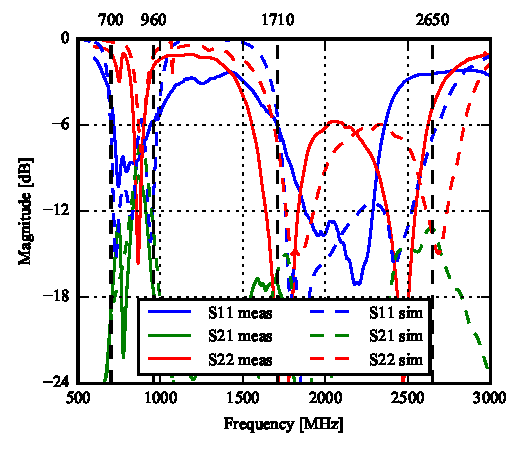
\includegraphics{img/tech_sol/nonresonant/prototype/sparams.pdf}
        \caption{S-parameters.}
    \end{subfigure}
    \hfill
    \begin{subfigure}{0.49\linewidth}
    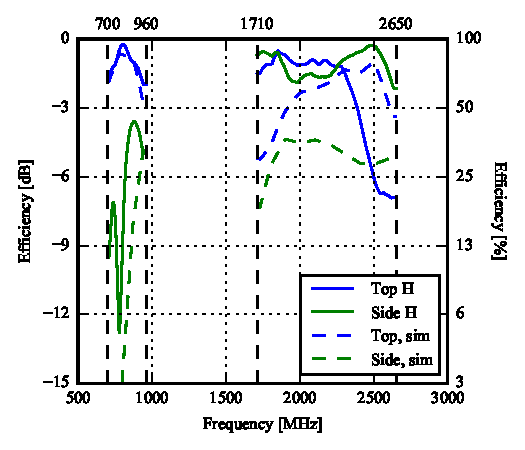
\includegraphics{img/tech_sol/nonresonant/prototype/eff_comp.pdf}
        \caption{Total efficiency.}
    \end{subfigure}
    \caption{S-parameters and total efficiency of the nonresonant antenna prototype with the component values from Figure~\ref{fig:ant3schematic_proto}.}
    \label{fig:nonresonant_proto_sparam_eff}
\end{figure}

   \begin{table}
      \centering
      \begin{tabular}{|l|l|r|r|r|}
        \hline
        Antenna & Band & Start [MHz] & Stop [MHz] & Bandwidth [MHz] \\
        \hline
        Top     & Low  & 700        & 960       & 260 \\
        Side    & Low  & 830         & 910        & 80 \\
        \hline
        Top     & High & 1710        & 2350       & 640 \\
        Side    & High & 1550        & 2645       & 1095 \\
        \hline
      \end{tabular}
      \caption{Maximum bandwidth obtained in the low and high band for the top and the side antenna, respectively.}
      \label{tab:bw_sol3_proto}
    \end{table}

\begin{table}
  \centering
        \begin{tabular}{|l|l|l|l|l|l|l|l|l|}
            \hline
                         & $L_{l1}$       & $L_{l2}$        & $C_{l3}$      & $L_{l4}$       & $C_{h1}$       & $L_{h2}$      & $C_{h3}$      & $C_{h4}$    \\
            \hline
            Top antenna  & \SI{10}{nH}  & \SI{15}{nH}  & \SI{3}{pF} & \SI{5.6}{nH} & \SI{1.2}{pF} & \SI{7.5}{nH} & \SI{3}{pF} & \SI{0.1}{pF} \\
            Side antenna & \SI{10}{nH}  & \SI{16}{nH}  & \SI{6.8}{pF} & \SI{4.3}{nH} & \SI{0.7}{pF} & \SI{5.1}{nH} & \SI{2.2}{pF} & \SI{1.2}{pF} \\
            \hline
        \end{tabular}
        \caption{Component values}
        \label{fig:ant3schematic_proto}
\end{table}

The measured and simulated envelope correlation coefficient can be seen in Figure \ref{fig:nonresonant_proto_ecc}. In the high band the simulated and measured correlation is quite similar. However for the low band the simulated and measured results deviates. Comparing the correlation to the isolation loss \ref{fig:nonresonant_proto_sparam_eff} it is clear that correlation should be highest in the low band. The diviation in the low band results could be caused by the measurement placement of the antenna. The antenna should be placed in the same position for every measurement, which can be hard to accomplice, also as mentioned in the triangle feed prototype section \ref{sec:triang_proto}.   

\begin{figure}[htbp]
    \centering
    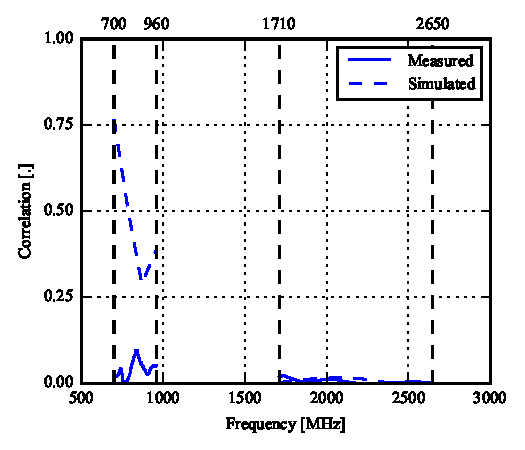
\includegraphics{img/tech_sol/nonresonant/prototype/correlation.pdf}
    \caption{Measured and simulated envelope correlation coefficient for the nonresonant antenna.}
    \label{fig:nonresonant_proto_ecc}
\end{figure}

\FloatBarrier
\section{Capacitor sweep}
The S-parameter sweep can be seen in Figure \ref{fig:nonresonant_proto_sweep_sparams}. The top antenna sweep S11 shows that the antenna is capable of covering the entire low band and most of the high band. In the high band the antenna have some problems from approx. \SI{2400}{MHz} to \SI{2650}{MHz}, as the return loss drops to approx. \SI{-3}{dB}. The results of the side antenna S22 shows that the antenna was unable to be tuned. Many component changes were made and it had no effect on the frequency tuning of the antenna. 
The highest isolation loss measured is \SI{-9}{dB} in the low band. In the high band the isolation loss is generally low with a max value of \SI{-14}{dB} over a bandwidth of approx. \SI{20}{MHz}. 

The efficiency sweep can be seen in Figure \ref{fig:nonresonant_proto_sweep_efficiency}. From the results it is seen, that the top antenna covers the low band quite well with an efficiency from \SI{70}{\percent} to \SI{95}{\percent}. However, in the high band the top antenna experiences some problems in the higher frequencies. The efficiency is approx. \SI{80}{\percent} from \SI{1710}{MHz} to \SI{2200}{MHz}, but drops to \SI{21}{\percent} from \SI{2200}{MHz} to \SI{2650}{MHz}. Generally tuning the top antenna results in an overall efficiency drop that is most significant in the higher frequencies.
As mentioned earlier the side antenna was unable to be tuned as the top so only one measurement of the side antenna efficiency were made. The efficiency results for the side antenna is therefore as described above in the comparison of the simulated and measured results.

tuning makes the efficiency to drop \fixme{Finish this}
\begin{figure}[htbp]
    \centering
    \begin{subfigure}{0.49\linewidth}
        \centering
        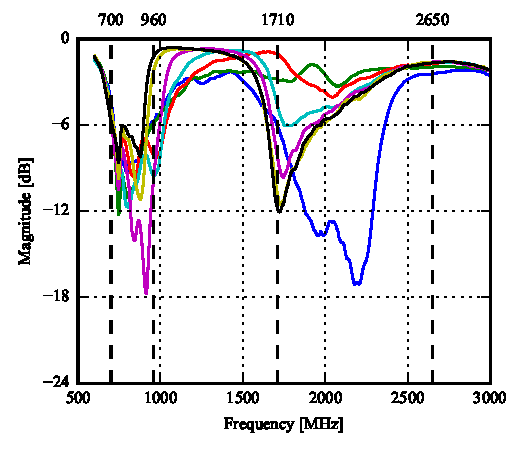
\includegraphics{img/tech_sol/nonresonant/prototype/s11_csh1.pdf}
        \caption{$S_{11}$, sweeping the top antenna and fixing the side antenna.}
    \end{subfigure}
    \hfill
    \begin{subfigure}{0.49\linewidth}
        \centering
        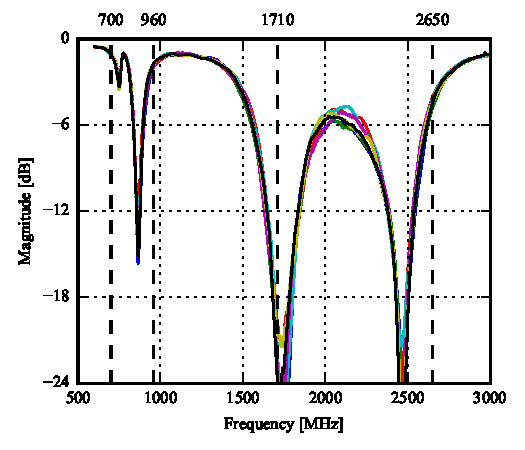
\includegraphics{img/tech_sol/nonresonant/prototype/s22_csh1.pdf}
        \caption{$S_{22}$, sweeping the top antenna and fixing the side antenna.}
    \end{subfigure}
    \\
    \begin{subfigure}{0.49\linewidth}
        \centering
        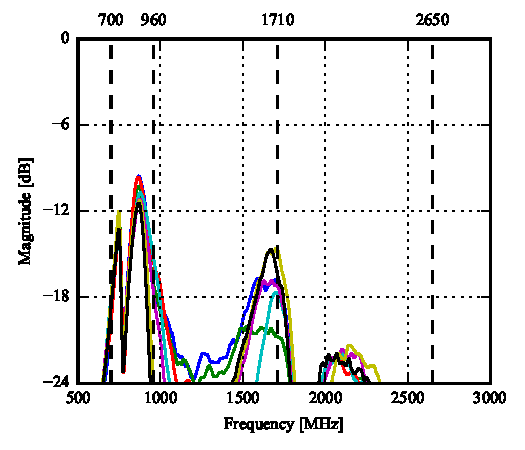
\includegraphics{img/tech_sol/nonresonant/prototype/s21_csh1.pdf}
        \caption{$S_{21}$, sweeping the top antenna and fixing the side antenna.}
    \end{subfigure}
    \caption{Non-resonant antenna. S-parameters for different shunt-capacitor values. The side antenna does not change resonance as desired when the shunt capacitor is changed. Therefore, only the top antenna is swept.}
    \label{fig:nonresonant_proto_sweep_sparams}
\end{figure}

\begin{figure}[htbp]
    \centering
    \begin{subfigure}{0.49\linewidth}
        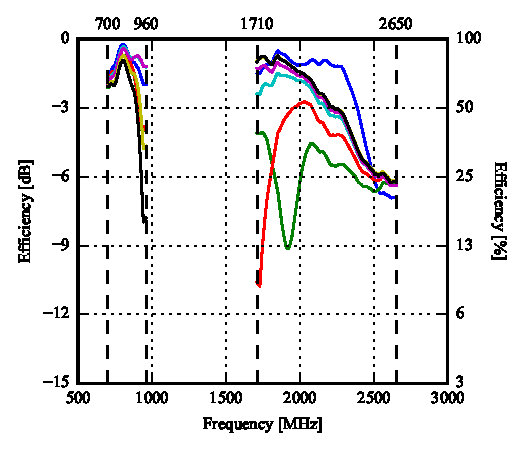
\includegraphics{img/tech_sol/nonresonant/prototype/efficiency_top.pdf}
        \caption{Top antenna, sweeping the top antenna and fixing the side antenna.}
    \end{subfigure}
    \hfill
    \begin{subfigure}{0.49\linewidth}
        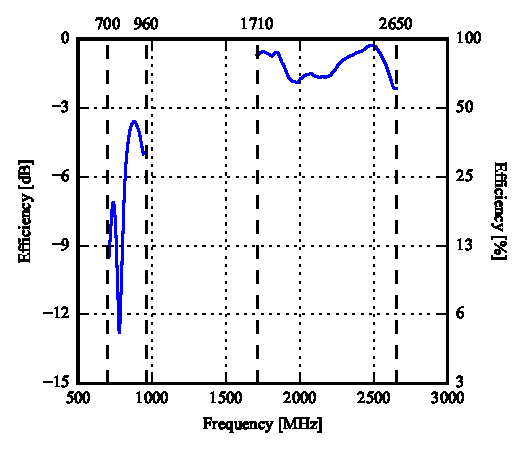
\includegraphics{img/tech_sol/nonresonant/prototype/efficiency_side.pdf}
        \caption{Side antenna, fixing both top and side antenna.}
    \end{subfigure}
    \caption{Total efficiency of both antennas when sweeping the top antenna. The side antenna does not sweep as desired when changing the capacitor. Therefore, no sweeps are made for the side antenna.}
    \label{fig:nonresonant_proto_sweep_efficiency}
\end{figure}
